\begin{minipage}{0.55\textwidth}
\begin{align*}
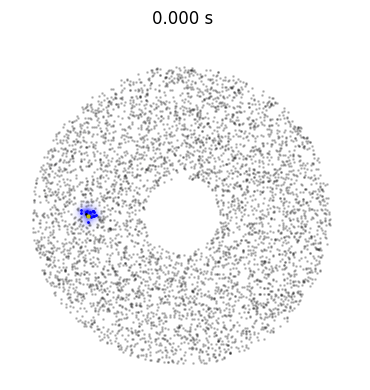
\includegraphics[width=0.49\textwidth]{simulation/1/frame_0.png}\hfill
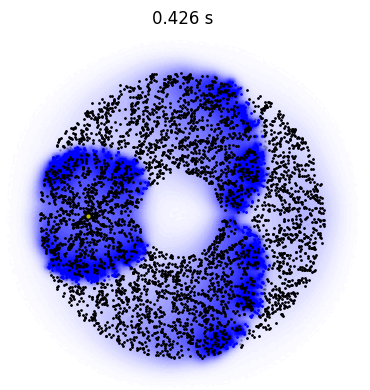
\includegraphics[width=0.49\textwidth]{simulation/1/frame_71.png}
\\[\smallskipamount]
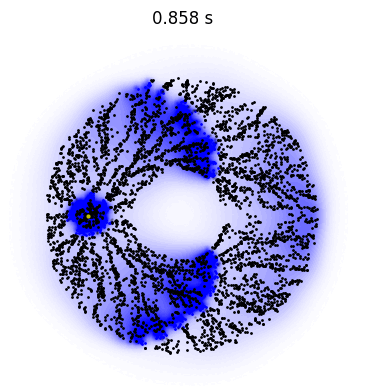
\includegraphics[width=0.49\textwidth]{simulation/1/frame_143.png}\hfill
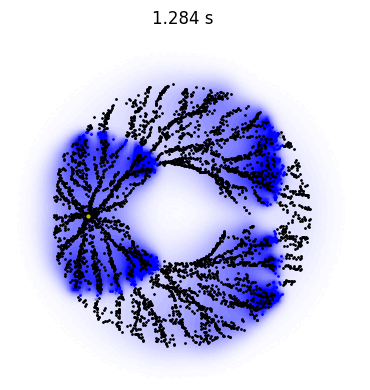
\includegraphics[width=0.49\textwidth]{simulation/1/frame_214.png}
\\[\smallskipamount]
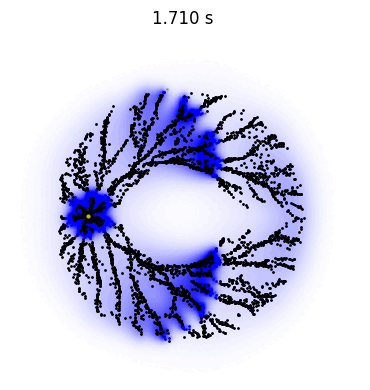
\includegraphics[width=0.49\textwidth]{simulation/1/frame_285.png}\hfill
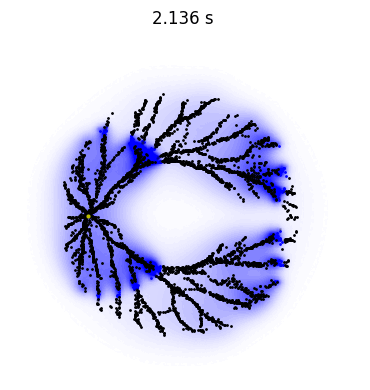
\includegraphics[width=0.49\textwidth]{simulation/1/frame_356.png}
\\[\smallskipamount]
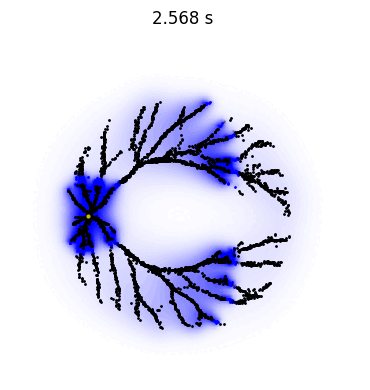
\includegraphics[width=0.49\textwidth]{simulation/1/frame_428.png}\hfill
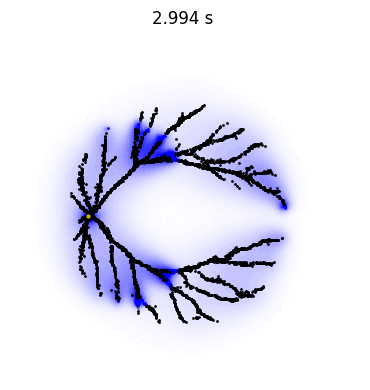
\includegraphics[width=0.49\textwidth]{simulation/1/frame_499.png}
\end{align*}
\end{minipage}
\begin{minipage}{0.45\textwidth}
\subsection{Annulus}
In our first simulation we used an uniform distribution on an annulus.
A pattern emerges after about $1$s.
It is apparent that the missing particles in the middle prevent any interaction through the hole which gives rise to branches above and below the hole, displaying a nice symmetry.
One can also observe that where the two \lq{}concentration fronts\rq{} collide on the right, a clear separation of the particles takes place.
\end{minipage}